%%%%%%%%%%%%%%%%%%%%%%%%%%%%%%%%%%%%%%%%%%%%%%%%%%%%%%%%%%%%%%%%%%%%%%%%%%% 
% 
% Generic template for TFC/TFM/TFG/Tesis
% 
% By:
% + Javier Macías-Guarasa. 
% Departamento de Electrónica
% Universidad de Alcalá
% + Roberto Barra-Chicote. 
% Departamento de Ingeniería Electrónica
% Universidad Politécnica de Madrid   
% 
% Based on original sources by Roberto Barra, Manuel Ocaña, Jesús Nuevo,
% Pedro Revenga, Fernando Herránz and Noelia Hernández. Thanks a lot to
% all of them, and to the many anonymous contributors found (thanks to
% google) that provided help in setting all this up.
% 
% See also the additionalContributors.txt file to check the name of
% additional contributors to this work.
% 
% If you think you can add pieces of relevant/useful examples,
% improvements, please contact us at (macias@depeca.uah.es)
% 
% You can freely use this template and please contribute with
% comments or suggestions!!!
% 
%%%%%%%%%%%%%%%%%%%%%%%%%%%%%%%%%%%%%%%%%%%%%%%%%%%%%%%%%%%%%%%%%%%%%%%%%%% 

\chapter{Predictive Techniques for Scene Understanding}
\label{cha:predictive_techniques}

\begin{FraseCelebre}
	\begin{Frase}
		Avanzad, sin temor a la oscuridad. \\
		Luchad jinetes de Theoden. \\
		Caerán las lanzas, se quebrarán los escudos. \\
		Aún restará la espada. \\
		Rojo será el día, hasta el nacer del sol. \\
		Cabalgad, cabalgad, cabalgad hacia la desolación \\ 
		y el fin del mundo. Muerte, muerte, muerte.
	\end{Frase}
	\begin{Fuente}
		Discurso de Theoden, Rey de Rohan \\
		El Señor de los Anillos: El Retorno del Rey
	\end{Fuente}
\end{FraseCelebre}

\section{Introduction}
\label{sec:4_introduction}

Autonomous driving has gained significant attention in recent years, with the development of intelligent vehicles and the increasing need for safe and efficient transportation systems. However, one of the main challenges in the field of autonomous driving is scene understanding, which involves the ability of a vehicle to recognize and interpret the objects and events in its environment. Accurate scene understanding is critical for safe and efficient driving, as it enables the vehicle to make informed decisions and take appropriate actions.

Deep learning has emerged as a powerful tool for scene understanding in autonomous driving, as it can automatically learn representations of complex and high-dimensional data. In particular, deep neural networks have shown remarkable performance in various tasks related to scene understanding, such as object detection, segmentation, and classification. However, the design and implementation of effective deep learning models for scene understanding in autonomous driving is still an active research area, and there is a need for more advanced predictive techniques to improve the performance of autonomous vehicles.

The main focus of this PhD thesis is to explore predictive techniques for scene understanding in autonomous driving using deep learning. The goal is to develop advanced models that can accurately recognize and interpret the objects and events in a vehicle's environment, and provide reliable predictions for safe and efficient driving. The thesis will investigate different deep learning architectures and techniques, such as convolutional neural networks (CNNs), recurrent neural networks (RNNs), and attention mechanisms, and evaluate their performance on various datasets and benchmarks. In addition, the thesis will investigate the use of transfer learning and domain adaptation to improve the generalization and robustness of deep learning models for scene understanding in diverse driving conditions and environments. The ultimate goal of this research is to contribute to the development of intelligent and safe autonomous driving systems that can operate effectively in real-world scenarios.

\section{SmartMOT}
\label{sec:4_smartmot}

% https://arxiv.org/pdf/2002.04849.pdf
% https://hal.science/hal-03347110/document
% https://www.mdpi.com/1424-8220/22/1/347

\subsection{Monitored Area Attention Module}
\label{subsec:4_maam}

AV need to locate itself in the environment to know what is happening close to it, in order to  make decisions and execute a correct navigation like a human driver would. When we talk about localization, the first thing we need is a map where to be located and, particularly for vehicles, this is road map. Road maps used by current navigators, e.g. Google Maps, are not valid for AV because of data type and the fact that they are not accurate enough to be used for autonomous driving. Here is where HD maps appear to solve this problem.

The concept of HD map is a text file describing the real-world features related to the road map and its location within a 2D/3D space,  and can do things that other sensors cannot \cite{wong2020mapping}: First, they have an "infinite range" and, therefore, can "see" even into occluded areas. Second, maps will never fail due to environmental conditions. Lastly, maps contain highly refined data. This information can be used by different modules of an AV, (including self-localization, vehicle control, path planning, perception and system management) drastically reducing the computational load and complexity in comparison to other more complex methods, providing robustness and reliability to the system.

\begin{figure}[] 
	\centering
	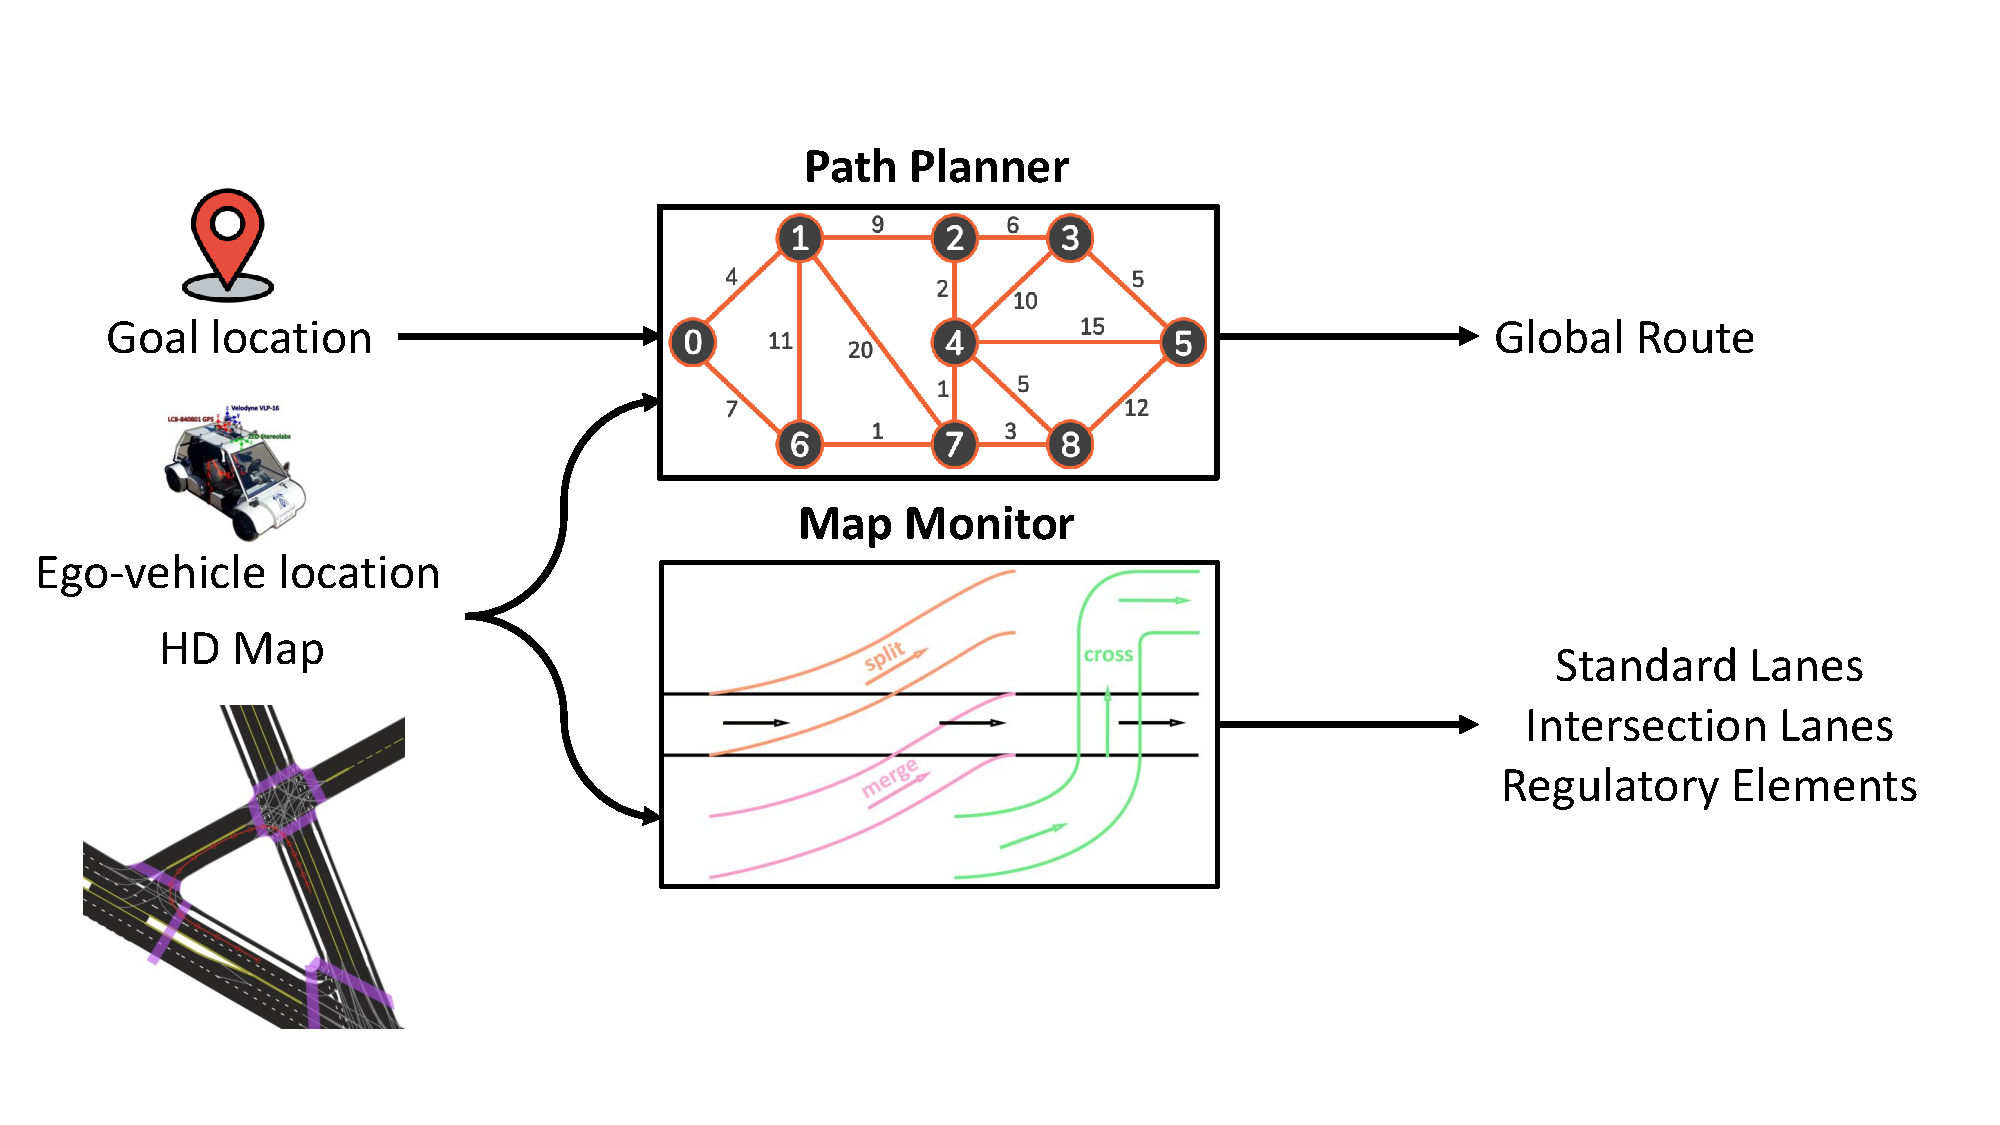
\includegraphics[width=0.8\textwidth]{figures/4_path_planner_map_monitor.pdf}
	\caption{Path Planning and Map Monitoring Outline}
	\label{fig:4_path_planner_map_monitor}
\end{figure}

There is not an standard definition about which data an HD map may include, but in the case of road maps, we could be talking about: roads, lanes, regulatory elements, topological information or any other information that can be considered relevant to drive in a safety way. HD map can be used to alleviate the computational load of other modules and add confidence to the real-world model. In our case, it is used for two different purposes, as illustrated in Figure \ref{fig:4_path_planner_map_monitor}: 

\begin{itemize}
	\item Global Path Planning, which uses a specific path planner which inputs are the HD map information and the ego-vehicle current location to retrieve an optimal (usually optimized based on the travelled distance) global route towards an specific goal.
	\item Map monitoring, responsible for monitoring the most relevant static and dynamic map elements around the ego-vehicle at each timestep, such as standard lanes (current, back), intersection lanes (merge, split and cross) and regulatory elements (e.g. give way, stop, pedestrian crossing, traffic light).
\end{itemize}



\section{GAN based Vehicle Motion Prediction}
\label{sec:4_gan_lstm}

\section{Exploring Map Features}
\label{sec:4_mapfe4mp}

We use the standard Negative Log-Likelihood (\textbf{NLL}) loss to train our social and map baselines in order to compare the ground-truth points $Y \in \mathbb{R}^{pred_{len} \times data_{dim}} = \{(x_0,y_0) ... (x_{pred_{len}}, y_{pred_{len}})\}$ with our multimodal predictions ($\hat{Y} \in \mathbb{R}^{k \times pred_{len} \times data_{dim}}$), given $k$ modalities (hypotheses) $\mathbf{p}=\{(\hat{x}^1_0,\hat{y}^1_0) ... (\hat{x}^k_{pred_{len}}, \hat{y}^k_{pred_{len}})\}$, with their corresponding confidences $\mathbf{c}=\{c_1 ... c_k\}$ using the following equation:

\begin{equation}
	\text{NLL} = -\log \sum_{k} e^{ \log{c^k} - \frac{1}{2} \sum_{t=0}^{pred_{len}} (\hat{x}^k_t - x_t)^2 + (\hat{y}^k_t - y_t )^2 }
	\label{eq:nll}
\end{equation}

\section{Leveraging traffic context via GNN}
\label{sec:4_mapfe4mp_gnn}

\begin{equation}
	$\mathcal{L}_{class,Hinge} = \frac{1}{(K-1)}\sum_{m=1 \setminus m \neq m^*}^{K} \max( 0, c_{k} + \epsilon - c_{m^*})$
\end{equation}

\section{Improving efficiency of Vehicle Motion Prediction}
\label{sec:4_cghformer}